\documentclass[aspectratio=169,11pt]{beamer}
% Reconstructed from the supplied PDF; standalone source with vector diagrams.
% All metrics are from the project case study and preserved experiment evidence.
\usepackage[T1]{fontenc}
\usepackage[utf8]{inputenc}
\usepackage{lmodern}
\usepackage{booktabs,array,amsmath,tikz}
\usetikzlibrary{arrows.meta,positioning,calc,shapes.geometric}
\geometry{paperwidth=192mm,paperheight=108mm}
\definecolor{navy}{HTML}{18344E}
\definecolor{teal}{HTML}{168578}
\definecolor{orange}{HTML}{CB7735}
\definecolor{slate}{HTML}{526779}
\definecolor{pale}{HTML}{EFF5F7}
\definecolor{rulegray}{HTML}{DBE4E9}
\setbeamercolor{normal text}{fg=navy,bg=white}
\setbeamercolor{structure}{fg=teal}
\setbeamercolor{frametitle}{fg=navy}
\setbeamercolor{block title}{fg=white,bg=navy}
\setbeamercolor{block body}{fg=navy,bg=pale}
\setbeamercolor{block title alerted}{fg=white,bg=orange}
\setbeamercolor{block body alerted}{fg=navy,bg=pale}
\setbeamerfont{frametitle}{size=\Large,series=\bfseries}
\setbeamerfont{block title}{size=\normalsize,series=\bfseries}
\setbeamersize{text margin left=8mm,text margin right=8mm}
\setbeamertemplate{navigation symbols}{}
\setbeamertemplate{itemize item}{\color{teal}\small$\bullet$}
\setbeamertemplate{itemize subitem}{\color{teal}\scriptsize$\bullet$}
\setbeamertemplate{frametitle}{\vspace{3mm}\insertframetitle\par\vspace{1mm}{\color{teal}\rule{\linewidth}{0.7pt}}}
\setbeamertemplate{footline}{\hspace{8mm}\color{slate}\scriptsize Lost in Transcription\hfill 3502\quad Principles of Machine Learning\hfill\insertframenumber\,/\,\inserttotalframenumber\hspace{8mm}\vspace{3mm}}
\setbeamertemplate{blocks}[rounded][shadow=false]
\newcolumntype{P}[1]{>{\raggedright\arraybackslash}p{#1}}
\setlength{\tabcolsep}{5pt}
\renewcommand{\arraystretch}{1.25}
\newcommand{\takeaway}[1]{\vfill\begin{beamercolorbox}[sep=2mm,wd=\linewidth]{block body}\small\textbf{Key point:} #1\end{beamercolorbox}}
\newcommand{\evidence}[1]{\vspace{1mm}\par{\tiny\color{slate}Evidence: #1\par}}
\newcommand{\metric}[2]{\begin{beamercolorbox}[sep=3mm,center,wd=\linewidth]{block body}{\LARGE\bfseries\color{teal}#1}\par\vspace{1mm}{\small #2}\end{beamercolorbox}}
\tikzset{box/.style={draw=rulegray,fill=pale,rounded corners=2pt,align=center,font=\small,inner sep=3mm}, dark/.style={box,draw=navy,fill=navy,text=white}, good/.style={box,draw=teal,fill=teal!8}, warn/.style={box,draw=orange,fill=orange!8}, flow/.style={-{Latex[length=2mm]},thick,draw=slate}, decision/.style={diamond,aspect=2.3,draw=teal,fill=teal!8,align=center,font=\small,inner sep=1mm}}
\hypersetup{pdftitle={Lost in Transcription: ASR Project Presentation},pdfauthor={Aakash Balasubramanian and Aniruth Devaraj},pdfsubject={3502 Principles of Machine Learning}}
\title{Lost in Transcription: ASR Project Presentation}
\author{Aakash Balasubramanian and Aniruth Devaraj}
\begin{document}

% 01
\begin{frame}[plain]
\vspace{5mm}
{\color{teal}\small\bfseries 3502\quad PRINCIPLES OF MACHINE LEARNING}\par
\vspace{7mm}
{\fontsize{29}{33}\selectfont\bfseries Lost in Transcription}\par
\vspace{3mm}
{\Large Indonesian--Javanese conversational ASR}\par
\vspace{5mm}
{\normalsize From a broad ensemble to a domain-adapted,\par conservatively fused offline system}\par
\vspace{6mm}
{\color{teal}\Large\bfseries Approximately 0.43 $\longrightarrow$ 0.2743 WER}\par
\vfill
{\normalsize\bfseries Aakash Balasubramanian \& Aniruth Devaraj}\par
\vspace{2mm}
{\small\color{slate}Project case study, methodology and implementation}\par
\vspace{5mm}
\end{frame}

% 02
\begin{frame}{Abstract and final outcome}
\begin{columns}[T]
\begin{column}{0.63\textwidth}
\textbf{Goal:} transcribe spontaneous code-switching speech while preserving colloquial words, disfluencies and reference spelling.
\vspace{3mm}
\begin{itemize}\item A broad pretrained ensemble looked strong locally but struggled on the leaderboard and runtime.
\item The pivot was to adapt a reliable Whisper Turbo anchor, then accept only supported corrections.
\item The final system used two Turbo checkpoints and adapted MERaLiON.
\end{itemize}
\end{column}
\begin{column}{0.32\textwidth}
\metric{0.2743}{Reported final competition WER}
\vspace{3mm}\metric{35.21\%}{Relative reduction: 0.4234 to 0.2743}
\vspace{3mm}\metric{30m 40s}{Measured CUDA inference}
\end{column}
\end{columns}
\takeaway{The achieved result belongs to the conservative Turbo system. Large-v3 is separate local research.}
\evidence{Submission history, supplied CUDA log and conservative archive inventory.}
\end{frame}

% 03
\begin{frame}{The problem: conversational speech under constraints}
\begin{columns}[T]
\begin{column}{0.49\textwidth}
\begin{block}{Recognition challenges}
\begin{itemize}\item Indonesian and Javanese switch within a clip.
\item Informal spelling, names and acronyms.
\item Fillers, repeats and interrupted words.
\item Conversational pauses and overlapping styles.
\item Training and hidden-test domains differ.
\end{itemize}
\end{block}
\end{column}
\begin{column}{0.47\textwidth}
\begin{block}{Engineering constraints}
\begin{itemize}\item Development on 16 GB Apple Silicon.
\item Offline execution on competition CUDA.
\item Hard inference limit: two hours.
\item Some target clips exceed 30 seconds.
\item Every clip processed independently.
\item Valid ordered CSV required for scoring.
\end{itemize}
\end{block}
\end{column}
\end{columns}
\takeaway{Semantic plausibility is insufficient: wording, coverage and reliable execution all affect the result.}
\end{frame}

% 04
\begin{frame}{Data audit and domain mismatch}
\begin{columns}[T]
\begin{column}{0.56\textwidth}
\small
\begin{tabular}{@{}lr@{}}\toprule
\textbf{Dataset / prepared split}&\textbf{Size}\\\midrule
Jember session recordings&208 MP3s\\
Original timestamped annotations&6,679 rows\\
Retained merged chunks&1,471\\
Jember train / holdout&1,309 / 162\\
Labelled competition clips&372\\
Conversation 5 / conversation 2&294 / 78\\\bottomrule
\end{tabular}
\vspace{3mm}\par
Jember: approximately \textbf{9.97 hours}.\par
Competition labelled audio: approximately \textbf{2.54 hours}.
\end{column}
\begin{column}{0.40\textwidth}
\textbf{Why direct transfer was hard}
\begin{itemize}\item Raw Jember median: 5 s; target: 26.01 s.
\item Jember is Javanese-heavy; target is mostly mixed speech.
\item 352 mixed, 20 Indonesian-only, no pure-Javanese target clips.
\item Prepared word-vocabulary coverage: 81.54\%; this is not a subword WER floor.
\end{itemize}
\end{column}
\end{columns}
\takeaway{Adapt duration and orthography while retaining the pretrained model's broader knowledge.}
\evidence{processed/v2 manifest, duration and vocabulary audits.}
\end{frame}

% 05
\begin{frame}{Preprocessing pipeline: auditable training examples}
\centering
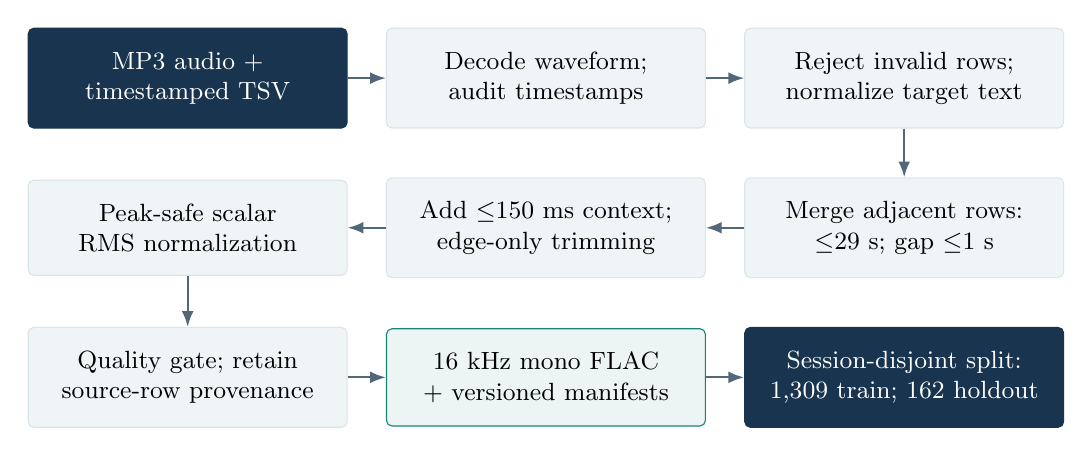
\begin{tikzpicture}[x=1cm,y=1cm]
\node[dark,text width=3.45cm] (a) at (0,0) {MP3 audio + timestamped TSV};
\node[box,text width=3.45cm] (b) at (4.55,0) {Decode waveform;\\audit timestamps};
\node[box,text width=3.45cm] (c) at (9.1,0) {Reject invalid rows;\\ normalize target text};
\node[box,text width=3.45cm] (d) at (9.1,-1.9) {Merge adjacent rows:\\$\leq$29 s; gap $\leq$1 s};
\node[box,text width=3.45cm] (e) at (4.55,-1.9) {Add $\leq$150 ms context;\\edge-only trimming};
\node[box,text width=3.45cm] (f) at (0,-1.9) {Peak-safe scalar\\ RMS normalization};
\node[box,text width=3.45cm] (g) at (0,-3.8) {Quality gate; retain\\ source-row provenance};
\node[good,text width=3.45cm] (h) at (4.55,-3.8) {16 kHz mono FLAC\\ + versioned manifests};
\node[dark,text width=3.45cm] (i) at (9.1,-3.8) {Session-disjoint split:\\1,309 train; 162 holdout};
\draw[flow] (a)--(b);\draw[flow] (b)--(c);\draw[flow] (c)--(d);
\draw[flow] (d)--(e);\draw[flow] (e)--(f);\draw[flow] (f)--(g);
\draw[flow] (g)--(h);\draw[flow] (h)--(i);
\end{tikzpicture}
\vspace{2mm}\par\small
\textbf{Stage accounting:} 6,679 rows $\to$ 6,638 valid $\to$ 1,472 merged $\to$ 1,471 retained.
\evidence{Versioned v2 preparation; 41 invalid rows and one final chunk removed.}
\end{frame}

% 06
\begin{frame}{Preprocessing choices: preserve speech, match the task}
\small
\begin{tabular}{@{}P{3.0cm}P{7.7cm}P{5.5cm}@{}}\toprule
\textbf{Stage}&\textbf{Implemented choice}&\textbf{Reason / boundary}\\\midrule
Text targets&Standardize punctuation and whitespace; remove Jember diacritics conservatively&Preserve casing, acronyms, fillers, repeats and word boundaries\\
Segmentation&Merge adjacent rows; pad boundaries; trim only edges&Match target duration without removing interior pauses\\
Audio scaling&RMS target $-23$ dBFS; peak cap $-1$ dBFS&Scalar gain, not denoising or a claim of better SNR\\
Quality audit&Check duration, silence and degeneracy; retain soft flags&Reject unusable examples without silently filtering hard speech\\
Inference audio&Decode float32; mono; resample to 16 kHz&Submitted Turbo/MER pipeline did not inherit training edge trimming or RMS scaling\\\bottomrule
\end{tabular}
\takeaway{Training targets, alignment keys and official scoring are separate text paths. Normalized alignment keys are not emitted as rewritten transcripts.}
\end{frame}

% 07
\begin{frame}{Evaluation: hold out entire conversations}
\begin{columns}[T]
\begin{column}{0.60\textwidth}
\centering
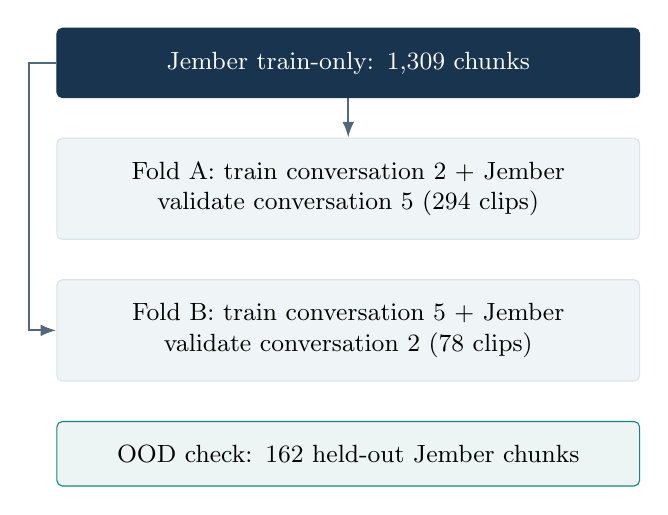
\begin{tikzpicture}[node distance=5mm]
\node[dark,text width=6.8cm] (j) {Jember train-only: 1,309 chunks};
\node[box,text width=6.8cm,below=of j] (a) {Fold A: train conversation 2 + Jember\\ validate conversation 5 (294 clips)};
\node[box,text width=6.8cm,below=of a] (b) {Fold B: train conversation 5 + Jember\\ validate conversation 2 (78 clips)};
\node[good,text width=6.8cm,below=of b] (h) {OOD check: 162 held-out Jember chunks};
\draw[flow] (j)--(a);\draw[flow] (j.west)--++(-.35,0)|-(b.west);
\end{tikzpicture}
\end{column}
\begin{column}{0.36\textwidth}
\textbf{Official-compatible metric}
\[\mathrm{WER}=\frac{S+D+I}{N}\]
\small
\begin{itemize}\item Aggregate = total errors / total reference words, not a fold average.
\item Report both folds and worst fold.
\item A clip oracle uses references to choose the best whole hypothesis; it is a diagnostic.
\item Conversation identity never routes inference.
\end{itemize}
\end{column}
\end{columns}
\takeaway{OOF reduces direct leakage, but repeated selection on only two conversations can still overfit.}
\end{frame}

% 08
\begin{frame}{Competition progression: adaptation made the largest step}
\centering
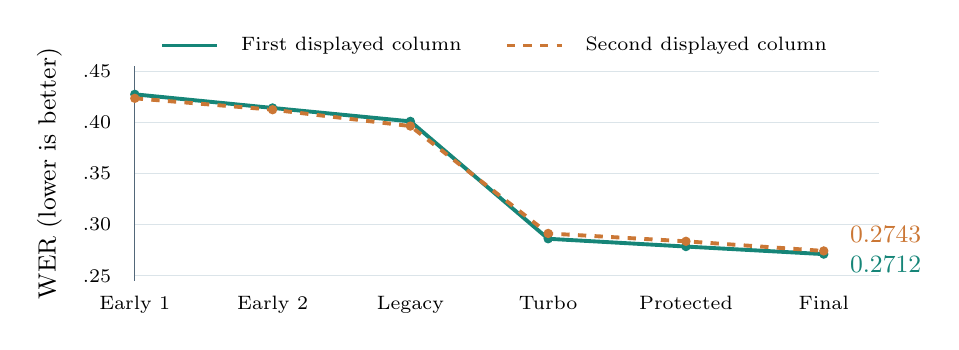
\begin{tikzpicture}[x=1.75cm,y=13cm]
\foreach \y in {.25,.30,.35,.40,.45}{\draw[rulegray] (0,\y)--(5.4,\y);\node[font=\scriptsize,anchor=east] at (-.1,\y) {\y};}
\draw[slate] (0,.245)--(0,.455);
\node[font=\small,rotate=90] at (-.62,.35) {WER (lower is better)};
\draw[teal,line width=1.4pt] (0,.4273)--(1,.4140)--(2,.4009)--(3,.2862)--(4,.2786)--(5,.2712);
\draw[orange,dashed,line width=1.4pt] (0,.4234)--(1,.4123)--(2,.3963)--(3,.2914)--(4,.2837)--(5,.2743);
\foreach \x/\y in {0/.4273,1/.4140,2/.4009,3/.2862,4/.2786,5/.2712}{\fill[teal] (\x,\y) circle (1.7pt);}
\foreach \x/\y in {0/.4234,1/.4123,2/.3963,3/.2914,4/.2837,5/.2743}{\fill[orange] (\x,\y) circle (1.7pt);}
\foreach \x/\t in {0/{Early 1},1/{Early 2},2/{Legacy},3/{Turbo},4/{Protected},5/{Final}}{\node[font=\scriptsize,anchor=north] at (\x,.24) {\t};}
\node[font=\small,teal,anchor=west] at (5.12,.261) {0.2712};
\node[font=\small,orange,anchor=west] at (5.12,.29) {0.2743};
\draw[teal,thick] (.2,.475)--(.6,.475);\node[font=\scriptsize,anchor=west] at (.7,.475) {First displayed column};
\draw[orange,dashed,thick] (2.7,.475)--(3.1,.475);\node[font=\scriptsize,anchor=west] at (3.2,.475) {Second displayed column};
\end{tikzpicture}
\vspace{3mm}\par\small
\textbf{Same-column reduction:} 0.4234 $\to$ 0.2743 = 0.1491 absolute, \textbf{35.21\% relative}.
\takeaway{0.2712 and 0.2743 belong to the same submission row. They are not two successive models.}
\evidence{Supplied screenshot; its column headers are cropped. Second column is the user's reported final result.}
\end{frame}

% 09
\begin{frame}{Initial exploration: many models, uneven usefulness}
\small
\begin{tabular}{@{}P{3.7cm}P{6.0cm}P{6.0cm}@{}}\toprule
\textbf{Model family}&\textbf{Role explored}&\textbf{Observed limitation}\\\midrule
Whisper Turbo / Large&Multilingual baseline; Indonesian/Javanese conditioning&Zero-shot wording and long-form handling needed attention\\
Qwen3-ASR-1.7B&Generalist candidate and ensemble hypothesis&MPS throughput/cache completion problems\\
MERaLiON&Conversational multilingual alternative&Useful errors, but naive voting was unreliable\\
Javanese XLS-R&CTC specialist for Javanese speech&Dtype and decoder API failures in early deployment\\
Buzz Javanese&Adaptive specialist and extra voter&Weak overall; useful on a limited subset\\
Medoid / ROVER&Select a transcript or vote aligned words&Local gains did not establish hidden robustness\\\bottomrule
\end{tabular}
\takeaway{These were evolving experiments, not one fixed six-model system deployed throughout the project.}
\end{frame}

% 10
\begin{frame}{Why the broad ensemble struggled}
\begin{columns}[T]
\begin{column}{0.48\textwidth}
\begin{block}{Measured or audited evidence}
\small\begin{itemize}\item Metadata-blind local ROVER: 0.205776; legacy leaderboard: 0.4009.
\item Metadata-aware replay: 0.206177. Routing alone did not explain the gap.
\item ROVER was worse than the best candidate on 153 clips; better on 98.
\item Early runs failed or exceeded two hours.
\item Audit found stale archive/config, long-form truncation and manifest-order risks.
\end{itemize}
\end{block}
\end{column}
\begin{column}{0.48\textwidth}
\begin{alertblock}{Plausible accuracy mechanisms}
\small\begin{itemize}\item Similar models can share wrong spelling or language preferences.
\item A weak voter can damage a stronger transcript.
\item Two conversations poorly represent the hidden domain.
\item Repeated local tuning can specialize the selector.
\item More model passes add runtime and deployment failure points.
\end{itemize}
\end{alertblock}
\end{column}
\end{columns}
\takeaway{No single cause of the hidden gap was proven. The next priority was a better anchor, not more votes.}
\evidence{Legacy replay, deployment audit and preserved platform observations.}
\end{frame}

% 11
\begin{frame}{The pivot: adapt Whisper Turbo with LoRA}
\begin{columns}[T]
\begin{column}{0.55\textwidth}
\small
\begin{tabular}{@{}ll@{}}\toprule
\textbf{Component}&\textbf{Implemented recipe}\\\midrule
Base&Whisper large-v3-turbo\\
LoRA&rank 32, alpha 64, dropout 0.05\\
Targets&Encoder + decoder attention / MLP\\
Trainable&27.85M / 836.73M (3.33\%)\\
Optimizer&AdamW, LR $3\!\times\!10^{-4}$\\
Local compute&MPS FP32; microbatch 1\\
Memory strategy&Accumulate 16; checkpoint gradients\\
Data sampling&Competition ratio 3 + Jember\\
Checkpointing&Half and full weighted epoch\\\bottomrule
\end{tabular}
\end{column}
\begin{column}{0.41\textwidth}
\centering
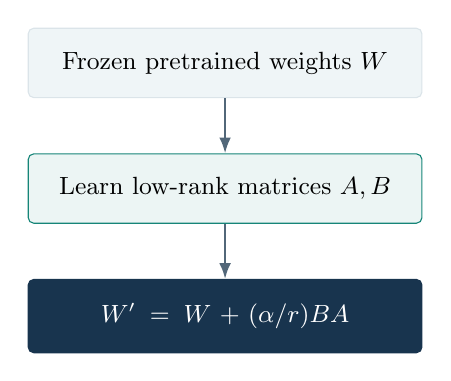
\begin{tikzpicture}[node distance=7mm]
\node[box,text width=4.4cm] (w) {Frozen pretrained weights $W$};
\node[good,text width=4.4cm,below=of w] (l) {Learn low-rank matrices $A,B$};
\node[dark,text width=4.4cm,below=of l] (o) {$W' = W + (\alpha/r)BA$};
\draw[flow] (w)--(l);\draw[flow] (l)--(o);
\end{tikzpicture}
\vspace{3mm}\par\small Retain broad acoustic knowledge while learning target-domain wording and switching patterns.
\end{column}
\end{columns}
\takeaway{Sampling ratio changes draw weights, not the number of independent labelled recordings.}
\end{frame}

% 12
\begin{frame}{Turbo experiments: inspect both folds}
\centering\small
\begin{tabular}{@{}llrrrr@{}}\toprule
\textbf{Condition / ratio}&\textbf{Checkpoint}&\textbf{A}&\textbf{B}&\textbf{Aggregate}&\textbf{Jember}\\\midrule
Indonesian / 3&Half&0.2236&0.2042&0.2197&0.2750\\
Indonesian / 3&Full&0.2259&0.1890&0.2184&0.2456\\
Javanese / 3&Full&0.2709&0.1842&0.2533&0.2442\\
Automatic / 3&Full&0.2328&0.1873&0.2235&0.2450\\
Indonesian / 4&Full&0.2249&0.1808&0.2159&0.2600\\\bottomrule
\end{tabular}
\vspace{4mm}
\begin{itemize}\item Initial deployment used Indonesian ratio-3 half, prioritizing the worst fold.
\item Javanese full helped B but substantially damaged A.
\item Full ratio-3 later became the fusion anchor after repetition handling.
\item Turbo-only leaderboard: \textbf{0.2862 / 0.2914}, the largest visible improvement step.
\end{itemize}
\takeaway{A lower aggregate alone did not justify a less balanced language or sampling recipe.}
\evidence{Conversation-disjoint cached predictions; Jember column is the fold-model mean.}
\end{frame}

% 13
\begin{frame}{MERaLiON: adapt for complementary errors}
\begin{columns}[T]
\begin{column}{0.39\textwidth}
\textbf{Memory-efficient adaptation}
\small\begin{itemize}\item Decoder-only LoRA: r16 / alpha32.
\item Frozen speech encoder and projector; cached representations.
\item Answer-only loss; chunked vocabulary projection.
\item AdamW $10^{-4}$; microbatch 1, accumulation 16.
\item Nonfinite full attempt retained a usable half checkpoint; stable retry used later.
\end{itemize}
\end{column}
\begin{column}{0.57\textwidth}
\small
\begin{tabular}{@{}lrrr@{}}\toprule
\textbf{OOF system}&\textbf{A}&\textbf{B}&\textbf{Agg.}\\\midrule
Whisper half&.2236&.2042&.2197\\
MER zero-shot&.2875&.2292&.2756\\
MER adapted&.2266&.2208&.2254\\
Adapted pair oracle&\textbf{.1892}&\textbf{.1718}&\textbf{.1857}\\
Simple ROVER&.2185&.2151&.2178\\\bottomrule
\end{tabular}
\vspace{4mm}\par
\begin{alertblock}{Complementarity is not a fusion result}
The oracle improved both folds. Simple voting still made Fold B worse than Whisper alone.
\end{alertblock}
\end{column}
\end{columns}
\takeaway{MERaLiON became a supporter for justified edits, rather than an unrestricted replacement.}
\end{frame}

% 14
\begin{frame}{Final architecture: a protected Turbo anchor}
\centering
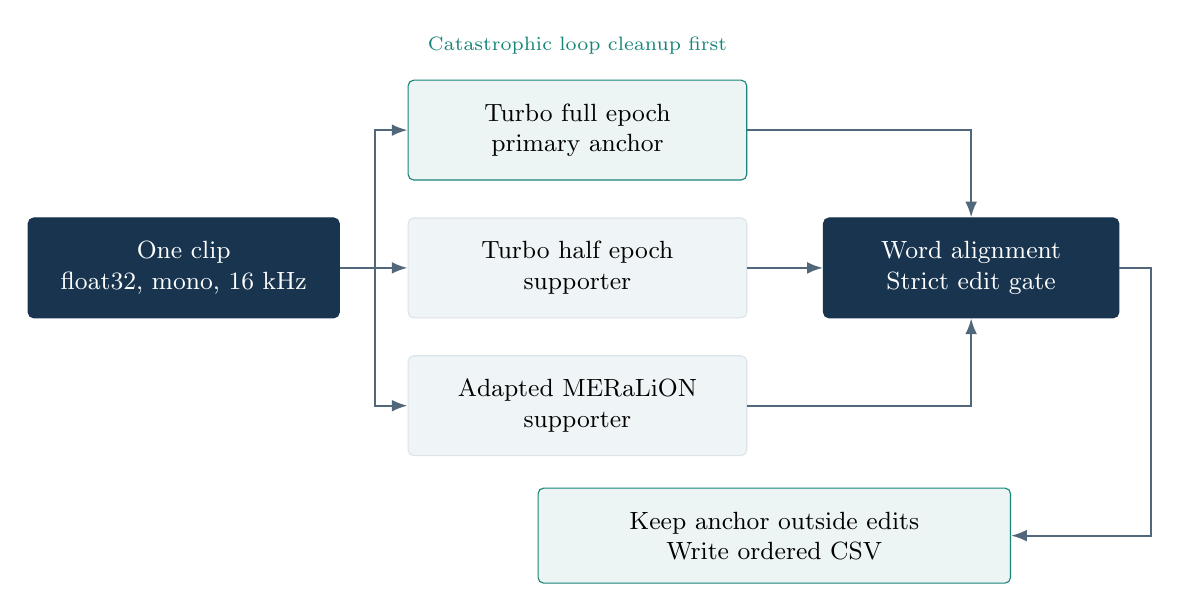
\begin{tikzpicture}[x=1cm,y=1cm]
\node[dark,text width=3.35cm] (in) at (0,0) {One clip\\ float32, mono, 16 kHz};
\node[good,text width=3.7cm] (full) at (5.0,1.75) {Turbo full epoch\\ primary anchor};
\node[box,text width=3.7cm] (half) at (5.0,0) {Turbo half epoch\\ supporter};
\node[box,text width=3.7cm] (mer) at (5.0,-1.75) {Adapted MERaLiON\\ supporter};
\node[dark,text width=3.15cm] (gate) at (10,0) {Word alignment\\Strict edit gate};
\node[good,text width=5.4cm] (out) at (7.5,-3.4) {Keep anchor outside edits\\Write ordered CSV};
\draw[flow] (in.east)--++(.45,0)|-(full.west);
\draw[flow] (in.east)--(half.west);
\draw[flow] (in.east)--++(.45,0)|-(mer.west);
\draw[flow] (full.east)-|(gate.north);
\draw[flow] (half.east)--(gate.west);
\draw[flow] (mer.east)-|(gate.south);
\draw[flow] (gate.east)--++(.4,0)|-(out.east);
\node[font=\scriptsize,text width=4.5cm,align=center,teal,above=2mm of full] {Catastrophic loop cleanup first};
\end{tikzpicture}
\takeaway{The three hypotheses are produced sequentially in deployment to control model residency.}
\end{frame}

% 15
\begin{frame}{Fusion gate: when is an edit allowed?}
\begin{columns}[T]
\begin{column}{0.53\textwidth}
\centering
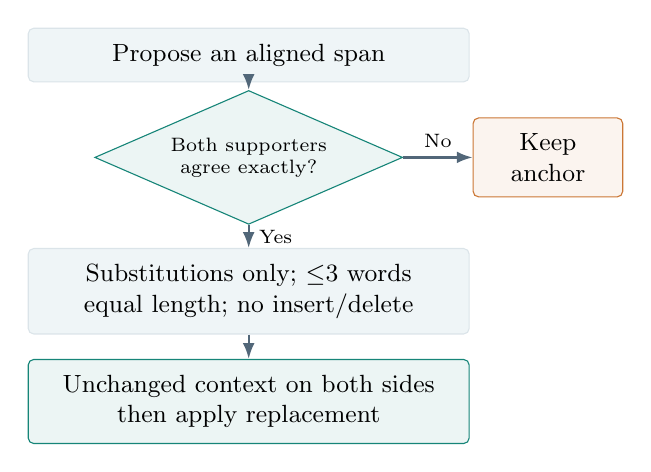
\begin{tikzpicture}[x=1cm,y=1cm]
\node[box,text width=5.2cm,inner sep=2mm] (p) at (0,0) {Propose an aligned span};
\node[decision,text width=2.1cm,font=\scriptsize] (a) at (0,-1.3) {Both supporters\\agree exactly?};
\node[box,text width=5.2cm,inner sep=2mm] (s) at (0,-3.0) {Substitutions only; $\leq$3 words\\equal length; no insert/delete};
\node[good,text width=5.2cm,inner sep=2mm] (c) at (0,-4.4) {Unchanged context on both sides\\then apply replacement};
\draw[flow] (p)--(a);\draw[flow] (a)--node[right,font=\scriptsize]{Yes}(s);\draw[flow] (s)--(c);
\node[warn,text width=1.5cm,inner sep=2mm] (n) at (3.8,-1.3) {Keep\\anchor};
\draw[flow] (a)--node[above,font=\scriptsize]{No}(n);
\end{tikzpicture}
\end{column}
\begin{column}{0.43\textwidth}
\textbf{Safeguards}
\begin{itemize}\item One weak model cannot override the anchor alone.
\item Reject unstable or repetitive MER support.
\item Use normalized keys for alignment; preserve original surface text elsewhere.
\item Single-word loops: five or more identical words collapse to two.
\item If cleanup changes indices, return the cleaned anchor without further edits.
\end{itemize}
\end{column}
\end{columns}
\takeaway{Ordinary fusion has no insertions or deletions; repetition cleanup is a separate operation.}
\end{frame}

% 16
\begin{frame}{Final selection: safer edits over a tiny OOF gain}
\centering\small
\begin{tabular}{@{}lrrrr@{}}\toprule
\textbf{Candidate}&\textbf{A}&\textbf{B}&\textbf{Aggregate}&\textbf{S / I / D}\\\midrule
Full Turbo, raw&.225860&.188976&.218359&--\\
Full Turbo, repetition-safe&.213296&.188976&.208350&--\\
A: broader operations&.208342&.185321&.203660&157 / 21 / 17\\
\textbf{B: strict substitutions}&\textbf{.209778}&\textbf{.185321}&\textbf{.204804}&\textbf{134 / 0 / 0}\\
C: confidence gate&.210281&.187289&.205605&97 / 13 / 12\\\bottomrule
\end{tabular}
\vspace{3mm}
\begin{columns}[T]
\begin{column}{0.48\textwidth}
\begin{block}{Why choose B?}
\small 61 fewer word edits than A; no ordinary insertions/deletions. Cost: only 0.001144 aggregate WER, with the same B result.
\end{block}
\end{column}
\begin{column}{0.48\textwidth}
\begin{block}{OOD sanity check}
\small Jember diagnostic: \textbf{0.244356} for B versus 0.245552 for full Turbo. No observed collapse.
\end{block}
\end{column}
\end{columns}
\takeaway{134 substitutions in 129 spans. Shared loop cleanup removed 196 words separately.}
\evidence{Official-compatible scorer. Jember uses fold-checkpoint means with final MER predictions; an OOD diagnostic, not OOF.}
\end{frame}

% 17
\begin{frame}{Error analysis: useful agreement can still be wrong}
\small
\begin{tabular}{@{}P{3.0cm}P{3.9cm}P{4.0cm}P{4.1cm}@{}}\toprule
\textbf{Example}&\textbf{Reference excerpt}&\textbf{Full Turbo}&\textbf{Fused excerpt}\\\midrule
Helpful spelling&beberapa kali pengen&beberapa kali pengin,&beberapa kali pengen,\\
Helpful word&udah kayak apa sih&udah layak, apa sih,&udah kayak apa sih,\\
Harmful variant&Nah, nggak seperti&Nah, nggak seperti&Nah, gak seperti\\
Harmful override&gitu loh tau gak tau&gitu lho. Tau gak tau&gitu lho. Aku gak tau\\\bottomrule
\end{tabular}
\vspace{4mm}
\begin{itemize}\item A supported correction can recover a reference spelling or wrong word.
\item Both supporters can agree on a plausible but incorrect alternative.
\item Reference-style orthography matters: \texttt{gak} and \texttt{nggak} can score differently.
\item Restricting edits reduces exposure; it does not guarantee correctness.
\end{itemize}
\takeaway{These are labelled OOF examples used for retrospective analysis, never hidden-test inference features.}
\evidence{Four saved OOF examples in docs/case\_study/error\_examples.json.}
\end{frame}

% 18
\begin{frame}{Deployment pipeline: offline and clip-independent}
\centering
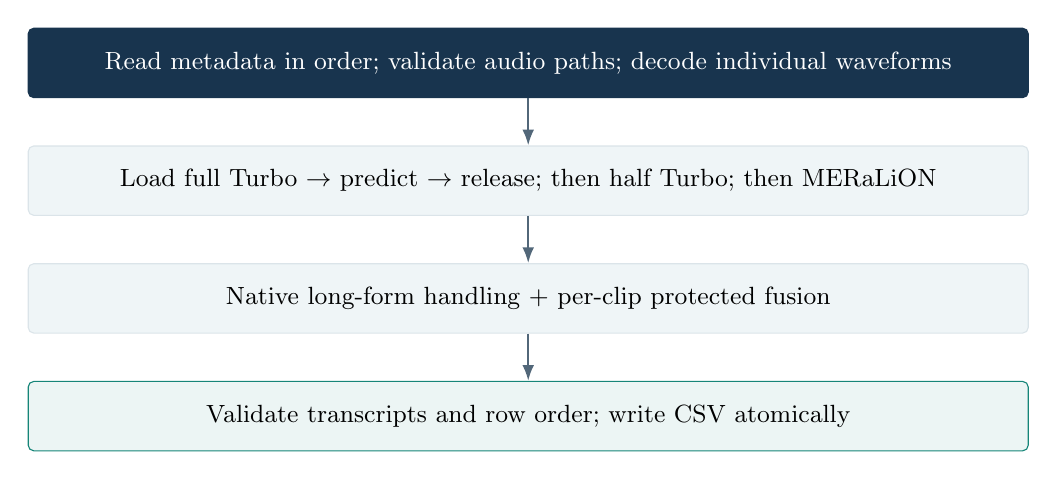
\begin{tikzpicture}[node distance=6mm]
\node[dark,text width=12.1cm] (meta) {Read metadata in order; validate audio paths; decode individual waveforms};
\node[box,text width=12.1cm,below=of meta] (load) {Load full Turbo $\to$ predict $\to$ release; then half Turbo; then MERaLiON};
\node[box,text width=12.1cm,below=of load] (fuse) {Native long-form handling $+$ per-clip protected fusion};
\node[good,text width=12.1cm,below=of fuse] (csv) {Validate transcripts and row order; write CSV atomically};
\draw[flow] (meta)--(load);\draw[flow] (load)--(fuse);\draw[flow] (fuse)--(csv);
\end{tikzpicture}
\vspace{3mm}\par\scriptsize
\textbf{Input:} \texttt{/code\_execution/data/test\_metadata.csv} and \texttt{data/clips/}\par
\textbf{Output:} \texttt{/code\_execution/submission/submission.csv}\par
\textbf{Schema:} \texttt{audio\_filename,transcript}\quad\textbf{CUDA batch:} 8\quad\textbf{MPS batch:} 1
\takeaway{All assets are bundled locally. Batching improves throughput without cross-test adaptation or transcript logging.}
\end{frame}

% 19
\begin{frame}{Verification: a model must finish and produce valid output}
\begin{columns}[T]
\begin{column}{0.52\textwidth}
\textbf{Checked on the packaged system}
\begin{itemize}\item Model loading with sockets blocked and empty external cache.
\item Normal clip: 21.60 seconds.
\item Long clip: 37.65 seconds; tail retained.
\item Repeated inference under fixed settings.
\item Exact CSV schema and sample order.
\item No blank or NaN failure rows.
\item ZIP integrity and SHA256 recorded.
\end{itemize}
\end{column}
\begin{column}{0.42\textwidth}
\metric{1,840.1 s}{Measured competition CUDA run}
\vspace{4mm}
\metric{Exit code 0}{submission.csv found by runner}
\vspace{4mm}\small
Archive: approximately \textbf{13.12 GB compressed}, 52 entries.\par
\vspace{2mm}Log inventory matches the local conservative package; the upload hash is absent from that log.
\end{column}
\end{columns}
\takeaway{Local smoke tests support correctness; the supplied CUDA completion log establishes successful platform execution.}
\evidence{Latest user-supplied log, archive inventory and preserved offline smoke checks.}
\end{frame}

% 20
\begin{frame}{Large-v3 follow-up: stronger local research, separate result}
\centering\small
\begin{tabular}{@{}lrrr@{}}\toprule
\textbf{Candidate}&\textbf{A}&\textbf{B}&\textbf{Aggregate}\\\midrule
Submitted conservative Turbo&.209778&.185321&.204804\\
Large-v3 full, standalone&.205542&.178009&.199943\\
Large-v3 supported consensus&\textbf{.199368}&\textbf{.172666}&\textbf{.193938}\\\bottomrule
\end{tabular}
\vspace{3mm}
\begin{columns}[T]
\begin{column}{0.48\textwidth}
\begin{block}{What worked locally}
\small r16 / alpha32, BF16 frozen base + FP32 LoRA, ratio 4. Half/full delta soups tested. Full retained for B/Jember balance; Turbo + MER supplied support.
\end{block}
\end{column}
\begin{column}{0.48\textwidth}
\begin{alertblock}{Generalization caution}
\small Final raw Jember WER: 0.265660. A multiword-loop safeguard improved the diagnostic. Beam and learned edit gates did not justify added complexity.
\end{alertblock}
\end{column}
\end{columns}
\takeaway{No supplied leaderboard result is attributed to this package. It did not produce the reported 0.2743.}
\evidence{Overnight and final nine-hour reports; preserved fold caches and checkpoint selection results.}
\end{frame}

% 21
\begin{frame}{Limitations and lessons}
\begin{columns}[T]
\begin{column}{0.48\textwidth}
\begin{alertblock}{Limits of the evidence}
\begin{itemize}\item Only two target conversations.
\item Repeated selection on the same folds.
\item No pure-Javanese target benchmark.
\item Jember is not the hidden distribution.
\item Agreement is not independent truth.
\item No established statistical significance.
\end{itemize}
\end{alertblock}
\end{column}
\begin{column}{0.48\textwidth}
\begin{block}{What changed the approach}
\begin{itemize}\item Improve the anchor before expanding fusion.
\item Audit data and deployment together.
\item Check both folds and edit aggressiveness.
\item Use oracles to diagnose, not claim deployable performance.
\item Preserve caches, checkpoints and hashes.
\item Keep recovery and runtime gates explicit.
\end{itemize}
\end{block}
\end{column}
\end{columns}
\takeaway{The local-to-hidden gap remains unresolved; the measured improvement does not prove every design choice caused it.}
\end{frame}

% 22
\begin{frame}{Conclusion and evidence trail}
\begin{columns}[T]
\begin{column}{0.62\textwidth}
\textbf{Delivered solution}
\begin{itemize}\item Versioned corpus preparation and official-compatible evaluation.
\item Domain-adapted Turbo full anchor with half-Turbo and MER support.
\item Conservative substitution gate and repetition protection.
\item A successful offline CUDA competition package.
\end{itemize}
\vspace{2mm}
\textbf{Next research step:} independent conversation validation for Large-v3 and its error corrections before claiming hidden robustness.
\end{column}
\begin{column}{0.34\textwidth}
\metric{0.4234 $\to$ 0.2743}{Same displayed score column}
\vspace{3mm}\metric{0.204804}{Submitted system local OOF WER}
\vspace{3mm}\small\color{slate}AI tools assisted research, coding and documentation; claims are grounded in saved experiment artifacts.
\end{column}
\end{columns}
\vfill
{\scriptsize\color{slate}\textbf{Evidence / references:} Project case study; processed/v2 manifest; fold caches; conservative selection report; latest CUDA log and submission screenshot.\par
\href{https://arxiv.org/abs/2106.09685}{Hu et al., LoRA (2021)}\quad$\cdot$\quad
\href{https://huggingface.co/openai/whisper-large-v3-turbo}{OpenAI Whisper Turbo model card}\quad$\cdot$\quad
\href{https://github.com/drivendataorg/lost-in-transcription-runtime}{DrivenData competition runtime}}
\end{frame}
\end{document}
